\documentclass{standalone}
%
\usepackage{tikz}
\usetikzlibrary{backgrounds,shapes.callouts}
\usepackage{tkz-euclide}
\usepackage{xcolor}
\usepackage{ifthen}
%
\definecolor{space}{HTML}{1F2C4E}
\definecolor{earth}{HTML}{0089FA}
\definecolor{dida}{HTML}{FFDE00}
\definecolor{title}{HTML}{FBA706}
\definecolor{moon}{HTML}{AFAFAF}
%
\usepackage{fontspec}
\setmainfont{Open Dyslexic}
%
\title{Una storia dell'universo}
\begin{document}
	\tikzset{
		partial ellipse/.style args = {#1:#2:#3}{insert path={+ (#1:#3) arc (#1:#2:#3)}},
		notice/.style  = { draw, ellipse callout, callout relative pointer={#1} },
	}
	\begin{tikzpicture}[background rectangle/.style={fill=white},show background rectangle,>={[inset=0,angle'=27]Stealth}]
		%title
		\draw [black,ultra thick] (1,1) rectangle (29,-1);
		\node at (15,0) {\textcolor{black}{\fontsize{40}{41}\selectfont Una storia dell'universo}};
		%\node at (15,11.8) {\textcolor{black}{\fontsize{90}{91}\selectfont del pioniere}};
		%
		\begin{scope}[shift={(0,-5)}]
			\node at (3,0) {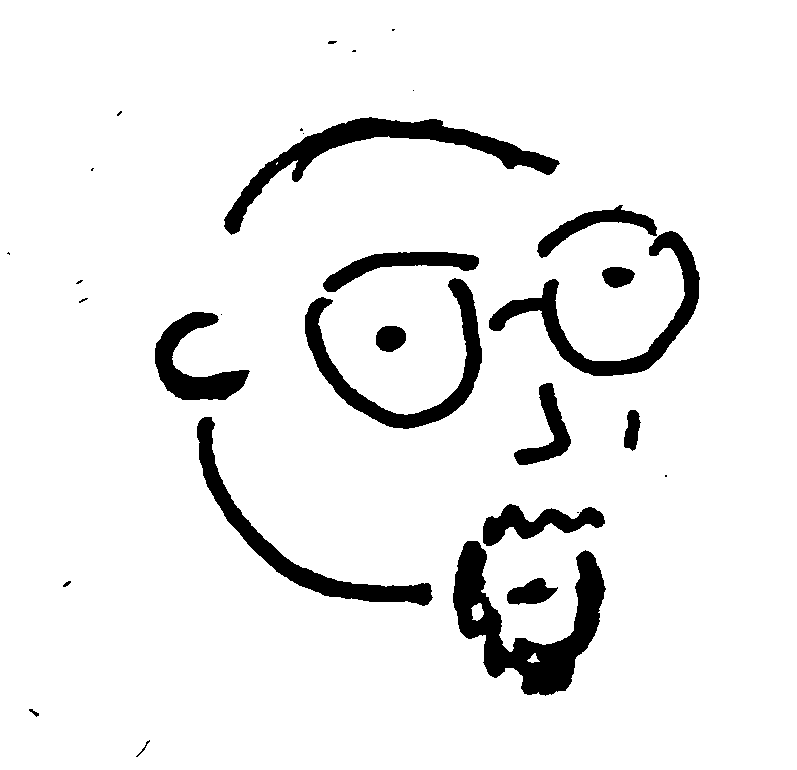
\includegraphics[width=5cm]{img-timeline/io_sx}};
			\node (example-textwidth-2) [right, align=left, text width=22cm, color=black, font=\fontsize{18pt}{19pt}\selectfont] at (6,0) {In un parco vicino a dove abito, a Milano, in un angolo un po' nascosto, c'e' una specie di timeline dell'universo che racconta dalla nascita fino a oggi la sua storia, mettendola in parallelo con lo scorrere dei 12 mesi.};
		\end{scope}
		% 
		\begin{scope}[shift={(0,-18)}]
			\node at (15,0) {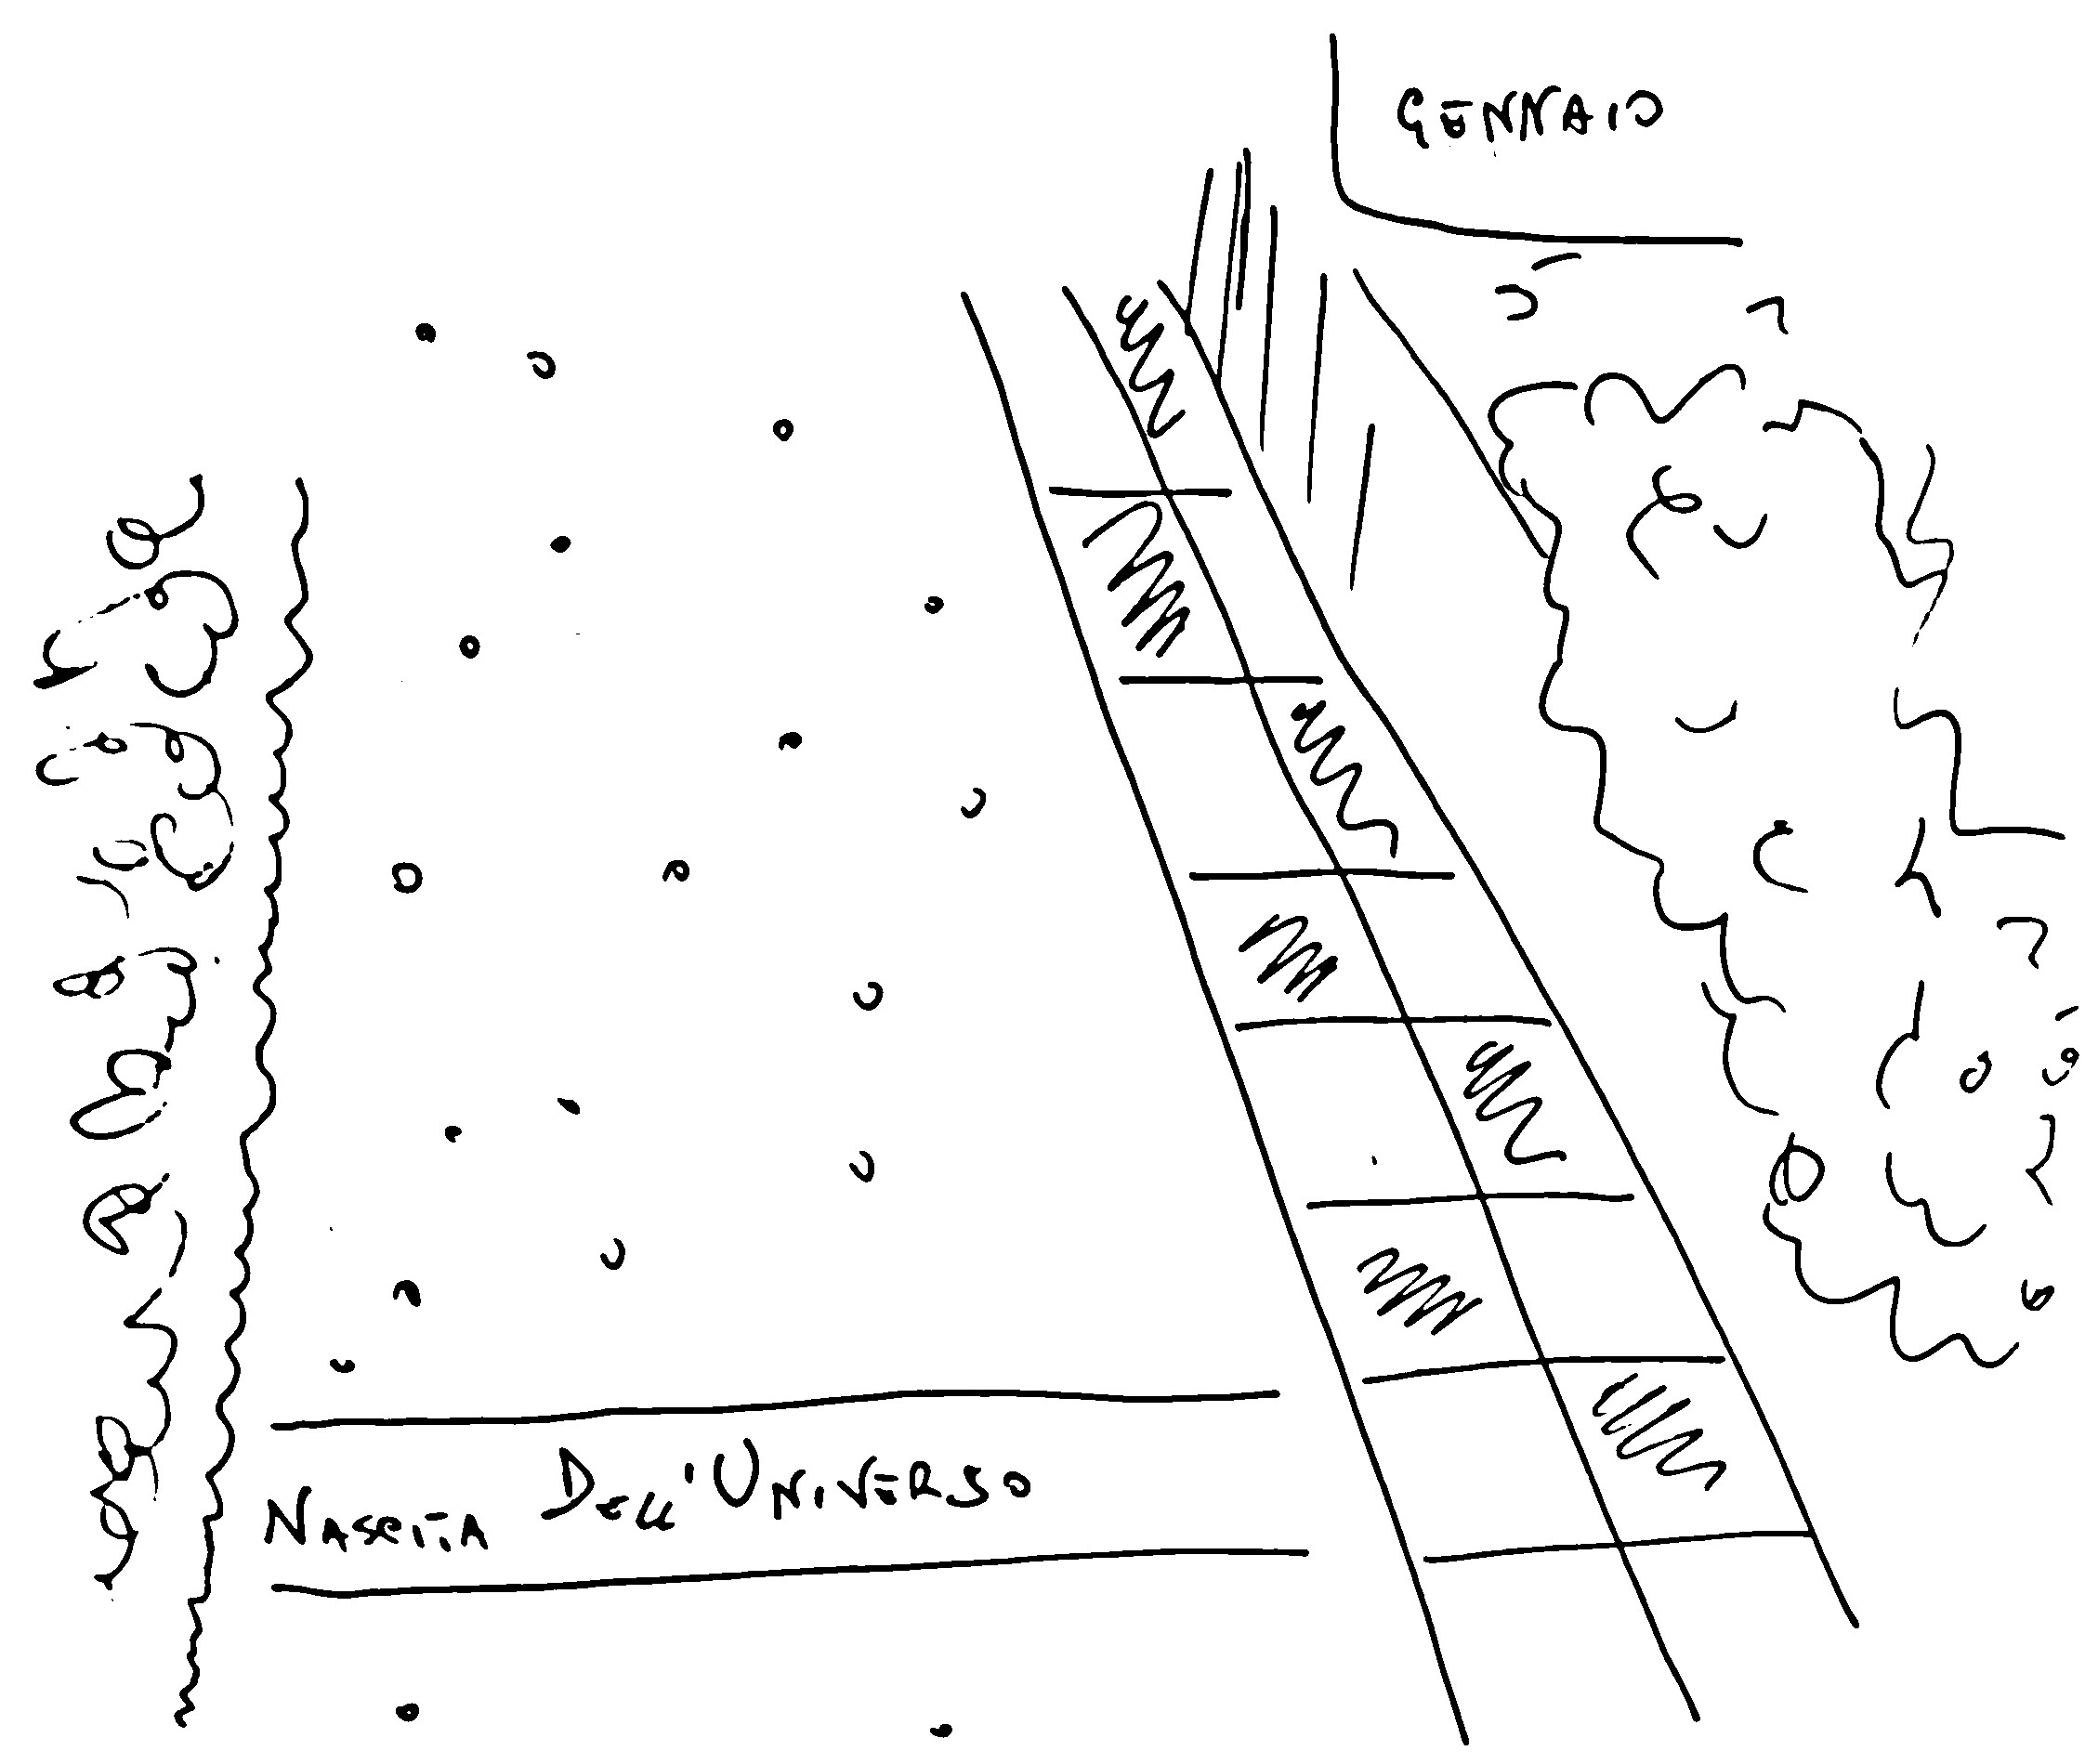
\includegraphics[width=25cm]{img-timeline/timeline_parco}};
		\end{scope}
		%
		\begin{scope}[shift={(0,-32)}]
			\node at (23,0) {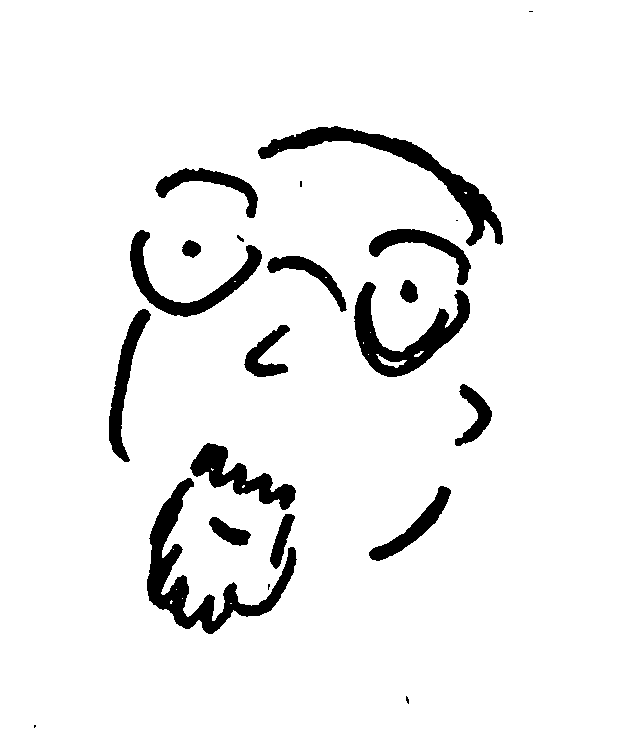
\includegraphics[width=5cm]{img-timeline/io_dx}};
			\node (example-textwidth-2) [right, align=left, text width=18cm, color=black, font=\fontsize{18pt}{19pt}\selectfont] at (2,0) {Personalmente l'ho trovata insoddisfacente, cosi' ho pensato di realizzare qualcosa di analogo anche io.};
		\end{scope}
		%
		\begin{scope}[shift={(0,-36)}]
			\draw[color=black,ultra thick] (3,0) -- (3,-48);
			\foreach \i in {0,1,2,...,12}
				\draw[color=black,ultra thick] (3,-\i*4) -- (3.2,-\i*4);
			\node at (4.8,0) {\textcolor{black}{\fontsize{14}{15}\selectfont 1 gennaio}};
			\node at (5,-48) {\textcolor{black}{\fontsize{14}{15}\selectfont 31 dicembre}};
			\draw[->,color=black,ultra thick] (6.5,0) -- (15,0);
			\draw[->,color=black,ultra thick] (6.5,0) -- (15,-1);
			\draw[->,color=black,ultra thick] (6.5,-0.001) -- (15,-5);
			\draw[->,color=black,ultra thick] (6.5,-0.26) -- (15,-7);
			\draw[->,color=black,ultra thick] (6.5,-0.35) -- (15,-10);
			\draw[->,color=black,ultra thick] (6.5,-1.7) -- (15,-13);
			\draw[->,color=black,ultra thick] (6.5,-17.4) -- (15,-17.4);
			\draw[->,color=black,ultra thick] (6.5,-24) -- (15,-24);
			\node at (20,0) {\textcolor{black}{\fontsize{14}{15}\selectfont Inizia l'espansione dello spaziotempo}};
			\node at (20.9,-1) {\textcolor{black}{\fontsize{14}{15}\selectfont Inizia l'era dei fotoni: da 10 s a 370000 anni}};
			\node (example-textwidth-2) [right, align=left, text width=12cm, color=black, font=\fontsize{14pt}{15pt}\selectfont] at (15.1,-2.7) {Dopo 18000 anni e fino alla fine dell'era dei fotoni avviene la ricombinazione in cui si formano i primi atomi. I fotoni della radiazione cosmicadi fondo sono originati proprio nel corso di questa epoca.};
			\node (example-textwidth-2) [right, align=left, text width=12cm, color=black, font=\fontsize{14pt}{15pt}\selectfont] at (15.1,-5.5) {Inizia l'era oscura che si conclude 150 milioni di anni dopo il Big Bang. Forse.};
			\node (example-textwidth-2) [right, align=left, text width=12cm, color=black, font=\fontsize{14pt}{15pt}\selectfont] at (15.1,-8) {Inizia l'era della reionizzazione dell'idrogeno gassoso durante la quale la luce puo' finalmente viaggiare libera nell'universo. Da 200 milioni a 1 miliardo di anni dopo l'espansione iniziale.};
			\node (example-textwidth-2) [right, align=left, text width=12cm, color=black, font=\fontsize{14pt}{15pt}\selectfont] at (15.1,-10.7) {Tra i 300 e i 400 milioni di anni dopo il Big Bang si formano le prime stelle e le prime galassie.};
			\node (example-textwidth-2) [right, align=left, text width=12cm, color=black, font=\fontsize{14pt}{15pt}\selectfont] at (15.1,-14.1) {Dopo 1 miliardo di anni dal Big Bang, si conclude l'era della reionizzazione e iniziano a formarsi le galassie che osserviamo oggi. Il processo prosegue per qualcosa come 9 miliardi di anni.};
			\node (example-textwidth-2) [right, align=left, text width=12cm, color=black, font=\fontsize{14pt}{15pt}\selectfont] at (15.1,-17.4) {Sono passati 10 miliardi di anni.};
			\node (example-textwidth-2) [right, align=left, text width=12cm, color=black, font=\fontsize{14pt}{15pt}\selectfont] at (15.1,-24.8) {Oggi, se consideriamo che l'universo e' \emph{nel mezzo del cammin della sua vita}. Siamo al 31 giugno seguendo il parallellismo con i 12 mesi. Da qui in poi non sappiamo bene cosa accadra'.};
		\end{scope}
		%
		\begin{scope}[shift={(0,-75)}]
			\draw[color=black,fill=white,ultra thick] (1,2) rectangle (29,-2);
			\node at (3,0) {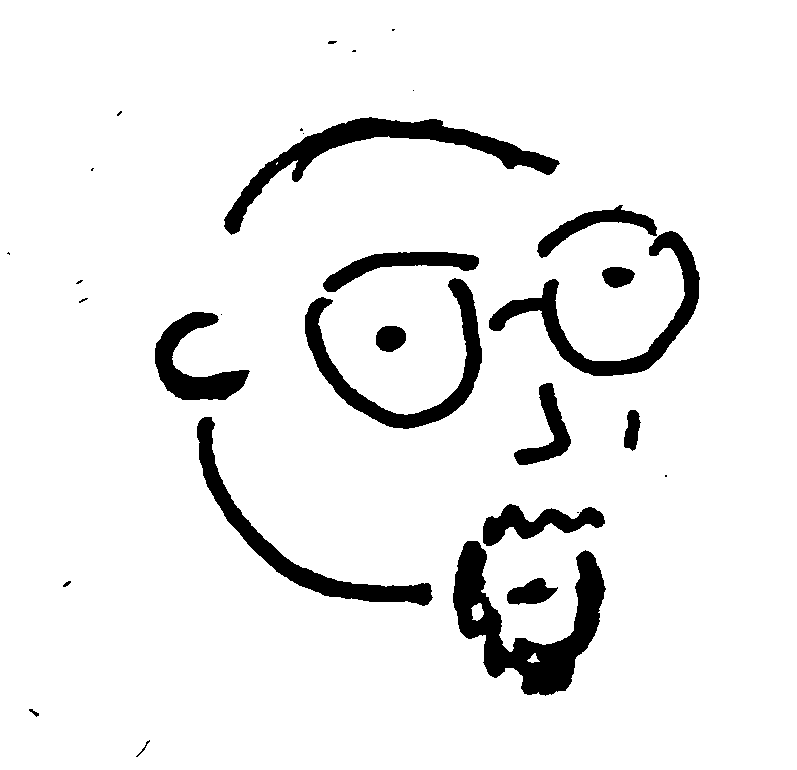
\includegraphics[width=5cm]{img-timeline/io_sx}};
			\node (example-textwidth-2) [right, align=left, text width=22cm, color=black, font=\fontsize{18pt}{19pt}\selectfont] at (6,0) {Potremmo quindi concludere che tutte le cose importanti nell'universo sono accadute in meno di un mese di tempo.\\O riprendendo l'analogia iniziale della passeggiata, nello spazio di un tallone umano!};
		\end{scope}
		%
		\begin{scope}[shift={(0,-86)}]
			\node at (27,0) () {
\includegraphics[width=3.7cm]{licenza}};
			\node at (18,-0.1) {\textcolor{black}{\fontsize{14}{15}\selectfont Testo e illustrazioni: @ulaulaman - Gianluigi Filippelli}};
		\end{scope}
	\end{tikzpicture}
%
\end{document}
